\documentclass[12pt, orivec]{article}
\usepackage{amsmath}
\usepackage{amssymb}     % for \rightsquigarrow
\usepackage{wasysym}
\usepackage[breakable]{tcolorbox}
\usepackage{ulem}
\usepackage{tikz-cd}		% commutative diagrams
\usepackage{tikz}
\usepackage{amsthm}
\usepackage[backend=biber,bibstyle=authoryear,citestyle=authoryearbrack]{biblatex}
\bibliography{../AGI-book}

\newtheorem{theorem}{Theorem}

\ifdefined\chinchin
\usepackage[CJKspace]{xeCJK}
\setCJKmainfont[BoldFont=SimHei,ItalicFont=AR PL KaitiM GB]{SimSun}
\newcommand{\cc}[2]{#1}
\else
\newcommand{\cc}[2]{#2}
\fi

\newcommand{\code}   [1]{{\footnotesize{\ttfamily #1}}}
\newcommand{\tab}{\hspace*{2cm}}
\newcommand{\powerset}{\raisebox{.15\baselineskip}{\Large\ensuremath{\wp}}}

\title{人工智能知识表述的数学基础}
\author{甄景贤}

\begin{document}
\setlength{\parindent}{0pt}
\setlength{\parskip}{2.8ex plus0.8ex minus0.8ex}

\maketitle

\section{什么是 model theory?}

举例来说,hyperbolic geometry(双曲几何)可以「实现」为某些 \textbf{模型}: 
\begin{equation}
\vcenter{\hbox{\includegraphics[scale=0.8]{hyperbolic-models.png}}}  \nonumber
\end{equation}
模型不是唯一的,可以有很多种。

在数理逻辑中,\textbf{模型论} 研究的是 syntax / \textbf{theory} 和 \textbf{model} 之间的 \textbf{对偶}。

First-order logic 的 模型 可以用一些 \textbf{集合} 及其 \textbf{元素} 组成。  例如,\\
$\mbox{John} \in \mbox{Male}, \quad \mbox{Mary} \in \mbox{Mathematician}$: 
\begin{equation}
\vcenter{\hbox{\includegraphics[scale=0.6]{FOL-model-1.png}}} 
\end{equation}
而 first-order objects(\textbf{个体})之间的 \textbf{关系} 是 domain $D$ 的 Cartesian product $D \times D$ 内的一些 \textbf{子集},例如:
\begin{equation}
\vcenter{\hbox{\includegraphics[scale=0.6]{FOL-model-2.png}}} 
\end{equation}

对计算系的人来说,更熟识的 model 是以下这种 relation graph 或 \textbf{knowledge graph}: 
\begin{equation}
\vcenter{\hbox{\includegraphics[scale=0.6]{FOL-model-3.png}}} 
\end{equation}
但这种 graph 不是数学中最常见的那种,因为它的 \textbf{边} 有 \textbf{labels}。 

以上的 knowledge graph 可以简单地转换成 \textbf{逻辑式子} 的集合:
\footnotesize
\begin{equation}
\begin{array}{l}
	\verb|Loves(John, Mary)| \\
	\verb|Loves(Pete, Mary)| \\
	\verb|Loves(Mary, Pete)| \\
	\verb|Hates(John, Pete)| \\
	\verb|Unhappy(John)|
\end{array}
\label{FOL-model}
\end{equation}
\normalsize
所以说,逻辑 与 graph 基本上是 \textbf{等价} 的。

如果 graph 的每条 边 可以包含任意个 顶点,则有 \textbf{hyper-graph}。 换句话说,hypergraph 的每条 边 $\in \powerset(V)$,$V$ 是 顶点集。 也可以说,hypergraph 就是 V 的 \textbf{子集系统} (set system)。  对逻辑来说,这好处是: \uline{关系 之上可以有 关系}。  

\begin{tcolorbox}
Hypergraph 可以一一对应於拓扑学上的 \textbf{simplicial complex},可以研究它的 homology 和 cohomology。 Simplicial complex 也可以和 \textbf{square-free monomial ideals} 一一对应。 后者是 \textbf{组合交换代数} (combinatorial commutative algebra) 的研究范围。  暂时我不知道这些关联有没有用,详细可参看 \parencite{Brown2013}, \parencite{Miller2005}。
\end{tcolorbox}

逻辑的 syntactic \textbf{theory} 方面,例如可以有以下这个式子(``失恋则不开心''):
\begin{equation}
\forall x,y. \; \mbox{Loves}(x,y) \wedge \neg \mbox{Loves}(y,x) \rightarrow \mbox{Unhappy}(x)
\end{equation}
这个式子含有 universal quantification,所以不是 model 的一部分。 逻辑上来说,只有 \textbf{ground sentences} (没有变量的式子)的集合才可以组成 model,例如 (\ref{FOL-model}) 。 

所以,\textbf{theory} 中的一个式子 可以导致 model 中出现很多 \textbf{新的} 顶点和连接。 这是 model theory 研究的问题。

\section{Categorical semantics}

\begin{equation}
\vcenter{\hbox{\includegraphics[scale=0.7]{logical-categories.png}}}
\end{equation}

\section{Domain theory}

\nocite{}
\printbibliography

\end{document}